\subsection{Cloud components in GeoCloud}

\subsubsection{Orchestrator}
\label{sub:orch}
The \emph{Orchestrator} is the
component that manages the tasks to be done in the cloud. It is running over the
\bonfire Cloud and controls all the interactions between all the components
implemented in the \bonfire testbed.

The \emph{Orchestrator} has the following functions:

\begin{itemize}
\item To identify which outputs shall be generated by the processors.
\item To generate the Job Orders. They contain all the necessary information
  that the processors need. Furthermore these \ac{XML} files include the interfaces and addresses of the folders in which the input information to the processors is located and the folders in which the outputs of the processors have to be sent. They also include the format in which the processors generate their output.
\item To look for raw data in the ground stations (pooling) to ingest such raw data in a shared storage unit in the cloud for its distribution to the processing chain.
\item To control the processing chain by communicating with the product processors.
\item To manage the archive and catalogue.
\end{itemize}

The orchestrator interacts with different modules:
\begin{itemize}

\item Ground stations implemented in \vw.
\item Processing instances in the cloud.
\item Archive and catalogue.
\end{itemize}

Figure~\ref{fig:orchestrator-interactions} depicts the \emph{Orchestrator’s} interactions with the other modules of the GEO-Cloud architecture.


\begin{figure}[!h]
\begin{center}
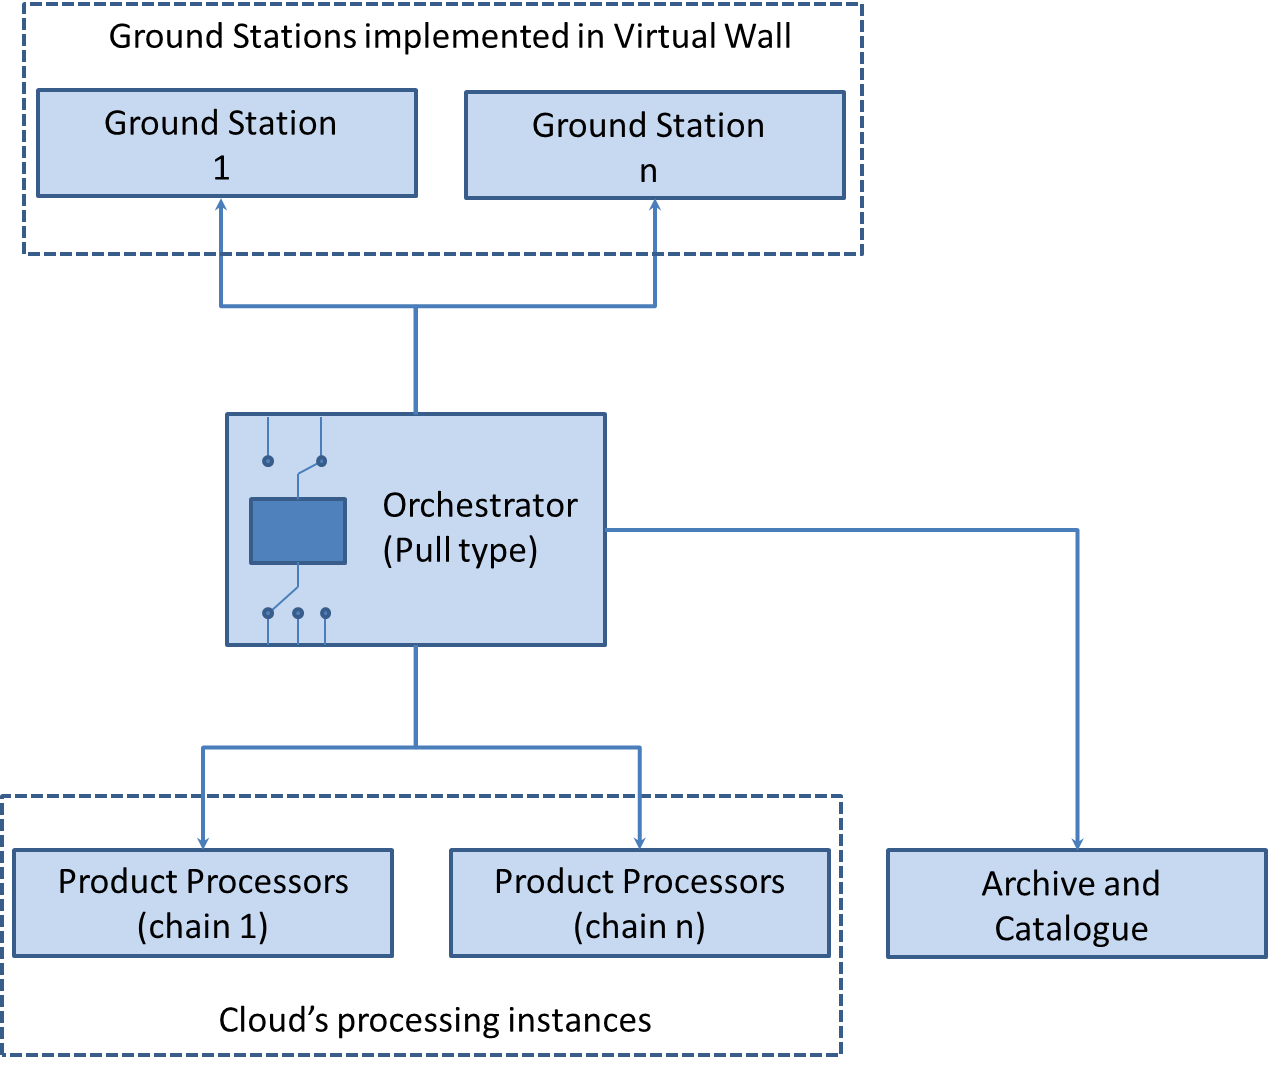
\includegraphics[width=0.7\textwidth]{cloud/orchestrator-interactions.png}
\caption{\emph{Orchestrator} interactions.}
\label{fig:orchestrator-interactions}
\end{center}
\end{figure}


As shown in Figure~\ref{fig:orchestrator-interactions}, the \emph{Orchestrator} is
pooling the Ground Stations frequently. When the \emph{Orchestrator} gets the data,
it uses the Product Processor for processing the data to generate the resulting
image. When this processing is finished, the \emph{Orchestrator} sends the image to
the \emph{Archive and Catalogue} to be available for customers.



\subsubsection{Processing Chain}
\label{subsub:processors}

The \emph{Processing Chain} is a module which is in charge of the processing of the
payload raw data from the satellites to produce image products. The four most
important operations that the product processors perform on the input data are
the following:
\begin{itemize}
\item A calibration, to convert the pixel elements from instrument digital counts into radiance units.
\item A geometric correction, to eliminate distortions due to misalignments of the sensors in the focal plane geometry.
\item A geolocation, to compute the geodetic coordinates of the input pixels.
\item An ortho-rectification, to produce ortho-photos with vertical projection, free of distortions.
\end{itemize}

The previous steps also generate quality-related figures of merit that are made
available in all the products. Moreover, the product processors generate
metadata, in line with industry standards, to facilitate the cataloguing,
filtering and browsing of the product image collection. These processors are
considerated as black boxes because they are owned by Elecnor Deimos and their
design and implementation can not be published, but them were studied for
carrying out this project.

The output image products are classified into four different levels, according to the degree of processing that they have been subjected to (see Figure~\ref{fig:cloud-states-pp}):
\begin{itemize}

\item \emph{Level 0} products are unprocessed images, in digital count numbers.
\item \emph{Level L1A} products are calibrated products, in units of radiance.
\item \emph{Level L1B} products are calibrated and geometrically corrected products (ortho-rectified), blindly geolocated.
\item \emph{Level L1C} products are calibrated and geometrically corrected products (ortho-rectified), precisely geolocated using ground control points.
\end{itemize}

\begin{figure}[!h]
\begin{center}

\includegraphics[width=0.9\textwidth]{detaildesign/stages-pp.jpg}
\caption{Stages of the product processing.}
\label{fig:cloud-states-pp}
\end{center}
\end{figure}

\paragraph{The L0 Processor}~\\

The acquired data is organized into image sectors of predefined size and structure and converted in scenes. Scenes, as defined here, are used throughout the subsequent L1 levels. The size and configuration of the scene is not changed again in the processing chain, for this reason the scene definition is constant for all the L1 levels.

The inputs are the following:
\begin{itemize}
\item The Raw Data.
\item The configuration database.
\item The calibration database.
\end{itemize}
The outputs are the following:
\begin{itemize}
\item The L0 products.
\end{itemize}

\paragraph{The L1A Processor}~\\

The goal of Level 1A is to calibrate the scenes. The resulting images are given in units of radiance.
The L1A component works on the scenes that compound the L0 product, performing different transformations over pixel values to generate radiances.

The inputs to the L1A level are the following:
\begin{itemize}
\item One L0 scene.
\item The configuration database.
\item The calibration database.
\end{itemize}

The output is the following:
\begin{itemize}
\item The L1A product.
\end{itemize}

\paragraph{The L1B Processor}~\\

Level 1B implements the geolocation, resampling and packing.

The inputs to the L1B level are the following:
\begin{itemize}
\item The L1A product.
\item The configuration database.
\item The calibration database.
\end{itemize}

The outputs are the following:
\begin{itemize}
\item The L1B products.
\end{itemize}


\paragraph{The L1C Processor}~\\

The L1C processor performs the ortho-rectification of the L1B product using ground control points.

The inputs to the L1C level are the following:
\begin{itemize}
\item The L1B  product.
\item The calibration database.
\item The configuration database.
\end{itemize}

The output is the following:
\begin{itemize}
\item Orthorectified Images.
\end{itemize}




\subsubsection{Archive and Catalogue}
\label{sub:archive}

The \emph{Archive and Catalogue} is a shared space of memory between the
\emph{Orchestrator}, the product processors and the distribution of data. It has
a data acquisition component which manages the input data arriving to the
\emph{Archive and Catalogue}. The ingestion of data in this module is automatic.

In the \emph{Archive and Catalogue} module the processed images are stored and catalogued for their distribution.

The \emph{Archive and Catalogue} basically consists of the archive and the
catalogue sub-modules:
\begin{itemize}
\item The \emph{Archive} is constituted by optimized storages structure allowing managing a big amount of data, efficient storage and retrieval of any kind of file. The \emph{Archive} is organized in hierarchical levels of storage in order to provide a cost effective storage solution.

\item The \emph{Catalogue} stores an inventory database with the metadata of archive files. It allows the product process chain easiness to access to the metadata from the processed products.

\item For the added value services the catalog will be accessed by a \emph{Web Service}.

\item \ac{CSW} is a module with the \ac{CSW} standard for the catalogue (based on \ac{OGC} standard). For more information on \ac{CSW}, please refer to \ac{OGC} \emph{OpenGIS Implementation Specification 07-006r1} and the \ac{OGC} tutorial on \ac{CSW}. Through this standard the distribution of data is done.
\end{itemize}

\begin{figure}[!h]
\begin{center}
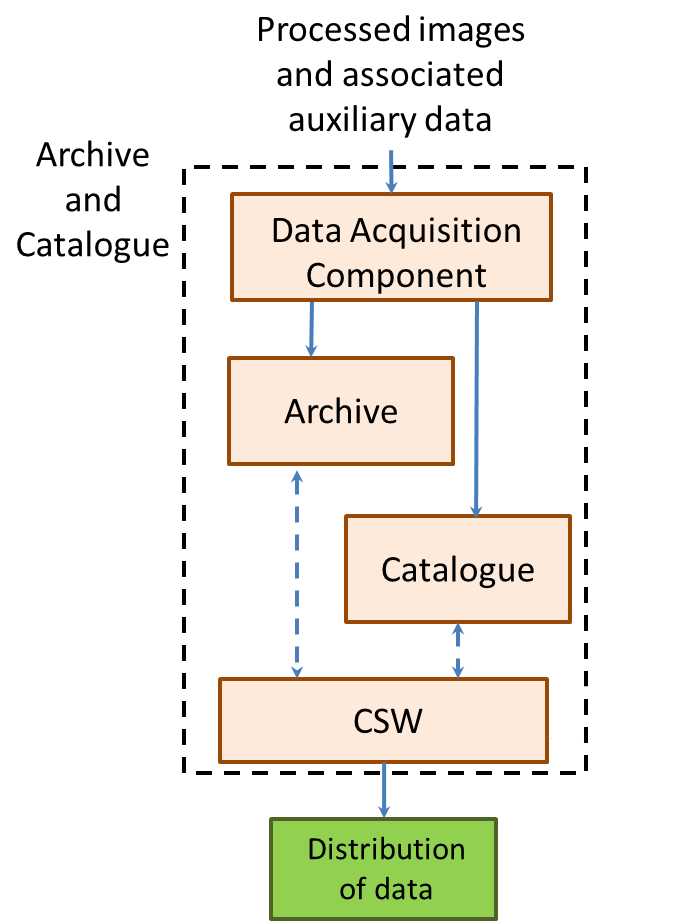
\includegraphics[width=0.5\textwidth]{detaildesign/scheme-archive-catalogue1.png}
\caption{Scheme of the \emph{Archive and Catalogue} module.}
\label{fig:archive-catalogue-scheme}
\end{center}
\end{figure}



\subsection{Implementation of the cloud architecture using SSH and SCP}
\label{subsec:ssh-cloud}
The cloud implementation using \ac{SSH} and \ac{SCP} is based in the following
components:
\begin{itemize}
\item The \emph{Orchestrator} module.
\item The \emph{Processing Chain} module.
\item The \emph{Archive and Catalogue} module.
\end{itemize}

The diagram in Figure~\ref{fig:first-architecture} shows the entire architecture is shown. The
communications were done using \ac{SSH} commands and the sending of the files were
performed using the \ac{SCP} protocol. For this implementation the raw data
travels from the \emph{Orchestrator} to the \emph{Processing Chain} module, where it is
processed. 
Finally, the Proccesing Chain module sends the processed image to the
Archive and
Catalogue module. 

It is important to highlight that the
\emph{Orchestrator} does not send the processed image to the \emph{Archive and Catalogue}
module, the \emph{Processing Chain} module sends it for archiving and cataloguing. Consecuently, the time for
archiving and cataloguing for each processed image was reduced.

\begin{figure}[!h]
\begin{center}
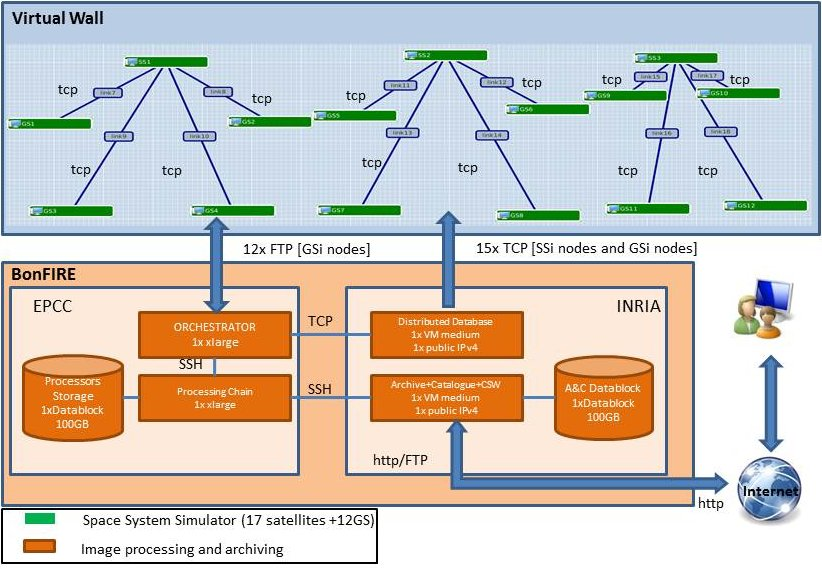
\includegraphics[width=1.0\textwidth]{cloud/first-architecture.jpg}
\caption{First architecture on cloud.}
\label{fig:first-architecture}
\end{center}
\end{figure}

The different components which compound the cloud architecture are fully
explained in the following sections. For each component, the  workflow, the
design, the implementation of the component and how was implemented in \bonfire are detailed.

\subsubsection{Implementation of the Orchestrator}

\paragraph{Orchestrator Workflow}~\\

The \emph{Orchestrator} component works by following the next sequence of steps:
\begin{enumerate}
\item The \emph{LoadData object} gets all the information about the \emph{Ground
    Stations Simulators} and localizes them.
\item The \emph{Listener object} pools to the \emph{Ground Stations} and when there are
  a downloadable raw data, the \emph{New\_Data\_Event} is launched.
\item  When the \emph{New\_Data\_Event} occurs, the \emph{Orchestrator} downloads the data.
\item  The \emph{Orchestrator} moves the raw data to a shared storage.
\item Then, the \emph{Orchestrator} makes different \emph{Job Orders} for the processors. The \emph{Job Order} contains all the useful information for the \emph{Product Processors} to proceed with the image processing.
\item The \emph{Orchestrator} gets the \emph{ProcessorChainController} object (this object was made regarding \emph{Singleton pattern}).
\item The \emph{Orchestrator} instructs the \emph{ProcessorChainController}
  object to create a new processing chain by sending the \emph{JobOrders}
  created in step 4. If there were any image processing, the request is queued.
\item The \emph{ProcessorChain Controller} object creates a new \emph{Processing
  Chain} to remotely process the data.
\item The \emph{Processing Chain} sequentially executes the L0, L1A, L1B, L1C processors.
\item When the \emph{ProcessingChain} has finished, this notifies the \emph{ProcessorChainController} object that the processing ended.
\item The \emph{ProcessingChainController} alerts the \emph{Orchestrator} that the \emph{Processing Chain} has finished.
\item The \emph{Orchestrator} takes the created image and puts it into the
  \emph{Archive}. As a improvement, this communication was not done. The
  sending to archiving and cataloguing is performed when the \emph{Processing Chain}
  finishes and sends the image to \emph{Archive and Catalogue} module. 
\end{enumerate}

Figure~\ref{fig:orchestrator-workflow} depicts the workflow of the \emph{Orchestrator}.

\begin{figure}[!h]
\begin{center}
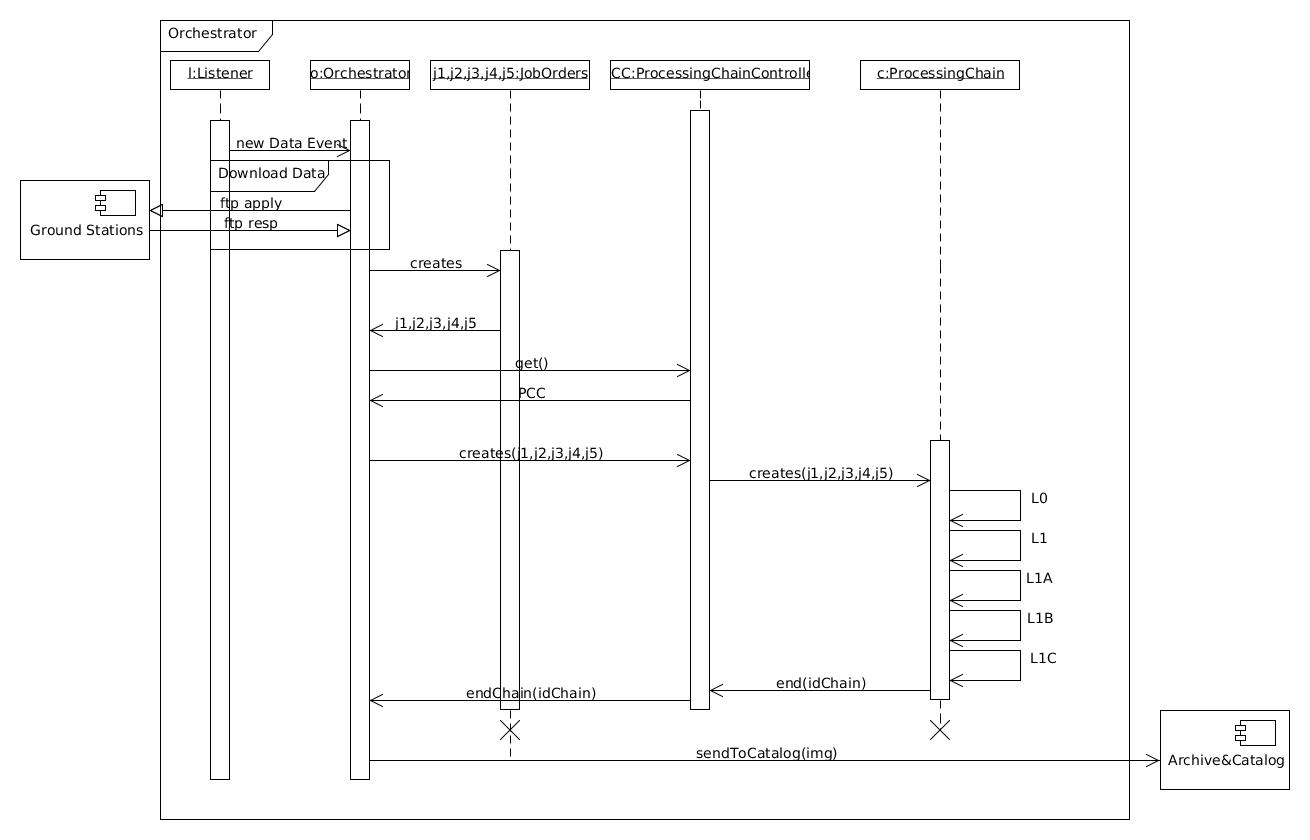
\includegraphics[width=1.0\textwidth]{cloud/orchestrator-workflow.jpg}
\caption{\emph{Orchestrator} workflow.}
\label{fig:orchestrator-workflow}
\end{center}
\end{figure}

\paragraph{Orchestrator Interfaces}~\\

The \emph{Orchestrator} has interfaces with the Ground Stations implemented in
\emph{Virtual Wall}, with the \emph{Product Processors} and with the
\emph{Archive and Catalogue}.
\subparagraph{Interfaces with the Ground Stations implemented in Virtual
  Wall}~\\

The \emph{Ground Stations} are deployed in some \emph{Virtual Wall} nodes. There, the impairments and features of the network are simulated. Essentially,
the \emph{Orchestrator} is pooling those \emph{Ground Stations} over \ac{FTP}
connections to know when new raw data is available. So, this Ground Stations are
\ac{FTP} servers in which the \emph{Orchestrator} can get the raw data obtained
by the constellation of satellites.

\subparagraph{Interfaces with the Product Processors}~\\

The \emph{Orchestrator} communicates with the \emph{Product Processors} through
the \emph{ProcessingChainController} instance as shown in
Figure~\ref{fig:orchestrator-workflow}. The \emph{Orchestrator} commands via
\ac{SSH} the \emph{ProcessingChainController} to create a new processing chains
to process the raw data and sends it through an \ac{SCP} transmission. \\
When this
process finishes, the \emph{ProcessingChainController} sends  a message to
indicate the end of the chain to the \emph{Orchestrator}. Thus, the
\emph{ProcessingChainController} checks the product processors progress and
initiates the next level until the processing chain finishes. Finally, the
\emph{Processing Chain} obtains the end product and locates it in the Catalogue service. 

\paragraph{Orchestrator Design}~\\

The Orchestrator is formed by the \emph{Listener}, the \emph{JobOrder} and
the \emph{ProcessingChainController}, the \emph{Orchestrator} and the \emph{Load} classes.

\begin{itemize}
\item \emph{Listener class}: It is responsible of obtaining the \emph{FTP}
  connections and polling them in order to get the images when they are created in the
  ground stations. When an image is detected in any ground station, a thread is
  created to download it. Then, the \emph{Orchestrator} object is signaled in order
  to begin the processing.
\item \emph{JobOrder class}: It perform the creation of the job orders. For
  simplicity, a specific job order is always used in all
  processings of scenarios.
\item \emph{ProcessingChainController class}: It  manages the processing in the
  product processors via \ac{SSH}. The processing is remotely executed. When an image is
  sent by the \emph{Orchestrator} class to the ProcessingChainController class, a
  new thread is created. Then, this thread remotely processes the image in the
  ProcessingChain module. If any request comes at same time, it is queued.
  This is a class based in the Singleton pattern.
\item \emph{Orchestrator class}: This class is designed by following a \emph{Controller}
  pattern. It manages the interactions between all above classes and integrates
  them.
\item \emph{LoadData class}: it parsers the configuration file for obtaining the
  \ac{IP} addresses of Database node, \emph{Archive and Catalogue} node and the
  \emph{Processing Chain} module. Furthermore, the user and password for \ac{FTP}
  connections are included into the configuration file. 
\end{itemize}



\paragraph{Orchestrator Implementation}~\\

The implementation of this module was done in Python 2.7. The libraries
needed to implement the software are listed in Table~\ref{table:orches-first-libraries}.

\begin{table}[hp]
  \centering
  {\small
  


\begin{tabular}{p{.2\textwidth}p{.2\textwidth}}
  \tabheadformat
  \tabhead{Python Library}   &
  \tabhead{Function}\\
\hline
\textit{Threading}         & System library for creating ,syncronizing and managing threads \\
\hline
\textit{OS}         & Library which provides operative system interactions \\
\hline
\textit{Collections}         & Library that contains the data structure
``deque'' used for queueing the request which can not be processed.\\
\hline
\textit{Time}         & For managing the time \\
\hline
\textit{Socket}         & Library for creating and establishing connections with other host \\
\hline
\textit{Pdb}         &  Used for debugging the software\\
\hline
\textit{FtpLib}         &Library used to obtain and manage the Ground Stations' FTP connections  \\
\hline
\end{tabular}


% Local variables:
%   coding: utf-8
%   ispell-local-dictionary: "castellano8"
%   TeX-master: "main.tex"
% End:

  }
  \caption{Orchestrator’s Python Libraries.}
  \label{table:orches-first-libraries}
\end{table}

Moreover, it requires the \ac{SCP} and \ac{SSH} clients for communicating  with other
modules in the cloud.
In addition, a script was developed in order to obtain the workload of the
\emph{Orchestrator} machine. That file uses the ``Python-psutil'' library in order to
obtain the CPU times such as user, idle, nice and iowait cycles. This file is
used by the graphical interface for plotting the workload of the \emph{Orchestrator} at
real time.


\paragraph{Orchestrator Execution}~\\

To execute the \emph{Orchestrator} module the following dependencies are required:
\begin{itemize}
\item Python v.2.7. For previous versions it has not been tested.
\item Python packages listed in Table~\ref{table:orches-first-libraries}.
\item Ethernet interface for the network connection in the \bonfire \emph{WAN}.
\item Connectivity with the database located in \bonfire through the network.
\item To setup the ``orchestrator.conf.xml'' with the correct \ac{IP} addresses
  of \emph{Archive and Catalogue} node, Chain Processing node and database node.
\end{itemize}

The execution of the satellite software it is executed inside the
``source/bonfire/orchestrator'' with the following
command line:
\begin{itemize}
\item[>] python main.py
\end{itemize}
 
\paragraph{Implementation in BonFIRE}~\\

For implementing of the \emph{Orchestrator} the following steps were done:

\begin{itemize}
 \item Reservation of a \emph{Xlarge} machine in \emph{EPCC} \bonfire
   platform. This machine belongs the \bonfire \emph{WAN} so it can communicate
   with all machines in that network. 
 \item Instalation of the necessary libraries (see
   Table~\ref{table:orches-first-libraries}).
 \item To upload the \emph{Orchestrator}' source to the \emph{Orchestrator} machine.
 \item To generate a pair of \ac{RSA} keys for enabling the connections to
   \emph{Procesing Chain} node.
\end{itemize}

\subsubsection{Implementation of the Processing Chain}

The implementation of the \emph{Processing Chain} was performed in a bash script. This script is remotely executed by the \emph{Orchestrator} for processing the
images. It was made in this manner because this is an implementation for testing the
processing behaviour on cloud. The elastic service provided by the \bonfire
platform was not available, so as a first approach, a machine was fixed for
testing the architecture.\\
 Furthermore, the clustering service provided for
\emph{INRIA} did not also work, so the dinamic creation of processes can not be
done because a only processing chain needs as minimum 6 GB of RAM memory. At the
end, only a Chain Processing at time can be executed, so this implementation is
very restricted in performance. 

\paragraph{Processing Chain Workflow}~\\

The \emph{Processing Chain} component works by following the next sequence of
steps:

\begin{enumerate}
\item The \emph{Orchestrator} component sends the image using \ac{SCP} to the
  directory ``tmp'' in the \emph{Processing Chain} machine.
\item The \emph{Orchestrator} remotely executes the script ``PP\_script.sh''
  located in the \emph{Processing Chain} machine.
\item The image processing start. The processors are sequentially executed.
\item When all the product processors have finished, the \emph{Processing Chain}
  sends the orthorectified image to \emph{Archive and Catalogue} using
  \ac{SCP}. 
\item The \emph{Processing Chain} orders the \emph{Archive and Catalogue} module
 to archive and catalogue the image received. In the first development, the
 \emph{Processing Chain} returned the results to the \emph{Orchestrator} and the
 orchestrator sent the images to the \emph{Archive and Catalogue} module for cataloguing
 and archiving. But that implementation was inefficient because there were two
 sending files more (the first one is between the \emph{Processing Chain} to the
 \emph{Orchestrator} and the second one, between the \emph{Orchestrator} and
 \emph{Archive and Catalogue}. Finally, the solution was to
 accomplish only a sending. The \emph{Processing Chain} after processing sends
 the results for archiving and cataloguing. 
\end{enumerate}

\paragraph{Processing Chain Interfaces}~\\

The \emph{Processing Chain} module has interfaces with both the \emph{Orchestrator}
and the \emph{Archive and Catalogue} modules.
\subparagraph{Interfaces with the Orchestrator}~\\

The \emph{Orchestrator} communicates with the \emph{Processing Chain} for
processing new incoming raw data. This communication is carried out using \ac{SCP} for file sending and for remote commands, (\ac{SSH}). This provides a manner of creating processes
on-demand. If the \emph{Processing Chain} machine was running in a cluster or
under an \ac{EaaS}, the
resources would be dinamically requested. 

\subparagraph{Interfaces with the Archive and Catalogue}~\\

The \emph{Archive and Catalogue} receives the images which the \emph{Processing
  Chain} has processed. The transfer of the images is performed using \ac{SCP}. Then, the
\emph{Processing Chain} remotely executes a Python script in the \emph{Archive
  and Catalogue} machine for archiving and
cataloguing the sent image.

\paragraph{Processing Chain Design}~\\

The \emph{Processing Chain} is formed by the ``PP\_script.sh'' bash
script. Originally, this module will be located in an \emph{EaaS}. The \bonfire
platform has not available this feature yet, so it was decided to push into a
cluster provided by the \emph{INRIA} testbed. The cluster platform was not also
available, so it was necessary to create and fix a machine which plays the
\emph{Processing Chain} role with the restriction that there can only be one
instance. 

\paragraph{Processing Chain Implementation}~\\
\label{par:pp-impl}
The implementation of this module was done using a bash script. This script needs the
\ac{IP} address of the \emph{Archive and Catalogue} module. In addition, it
requires the \ac{SCP} and \ac{SSH} clients for its interfaces with the other
modules. The image which is sent to the \emph{Archive and Catalogue} when the
process is finished, it is always the
same because for the experiment is more important the processing on cloud than
the resulting image.
  
In addition, a script was developed in order to obtain the workload of the
\emph{Orchestrator} machine. That file uses the ``Python-psutil'' library in order to
obtain the CPU times such as user, idle, nice and iowait cycles. This file is
used by the graphical user interface for plotting the workload of the \emph{Orchestrator} at
real time.

Finally,  shared storage was used to store the images instead of
the local storage. The shared storage is provided by the \emph{IBBT} testbed. This storage is implemented using \ac{NFS} protocol. Ideally, the \ac{NFS}
protocol using a network with a large bandwidth and links with 10 GB Ethernet is
more efficient than using a local hard disk. However the \ac{NFS}
server is not conformed by disks located in the \bonfire platform. The physical disks
where the information is saved are in \emph{IBBT} located in Ghent (Belgium). Thus, the
read and write accesses from any \bonfire testbed (INRIA and EPCC in this case)
travel from \bonfire to \emph{IBBT} through the Internet. This involves high
latencies, large waiting times and it implies that the CPU is idle large time
waiting for I/O operations. These results are shown in Section~\ref{sec:geocloud-results}.

The implementation of this shared storage was performed as follows:
\begin{itemize}
\item In the \bonfire web interface, a shared storage was created. 
\item The folders structure for processing were done. This structure is composed
  by (the local structure has the same distribution): 
\begin{itemize}
\item Job orders folder: it contains the job orders necessary for processing all
  stages.
\item l0\_input folder: it contains the neccesary inputs for L0 processor. 
\item l0r\_input folder: it contains the neccesary inputs for L0R processor. 
\item l1a\_input folder: it contains the neccesary inputs for L1A processor. 
\item l1br\_input folder: it contains the neccesary inputs for L1BR processor. 
\item l1bc\_input folder: it contains the neccesary inputs for L1BC processor. 
\item l1cr\_input folder: it contains the neccesary inputs for L1CR processor. 
\item l1ct\_input folder: it contains the neccesary inputs for L1CT processor. 
\end{itemize}
\item Processors outputs folder: contains the outputs and temporaly files
  created by the processors during their actions.
\end{itemize}

\paragraph{Processing Chain Execution}~\\

To execute the \emph{Processing Chain} module the following dependencies are
required:
\begin{itemize}
\item To know the \ac{IP} address of the \emph{Archive and Catalogue}.
\item Ethernet interface for the network connection in the \bonfire \emph{WAN}.
\item The geolocated image for sending to \emph{Archive and Catalogue} module
  once the processing is finished. 
\item The Product Processors owned by \emph{Elecnor Deimos} installed in the
  machine.
\end{itemize}

The script is located inside
``source/bonfire/ProcessingChain'' folder. The execution of the software is executed with the following
command line:
\begin{itemize}
\item[>] bash PPscript.sh <<arg1>> <<arg2>>
\end{itemize}
where \emph{arg1} is the outfile name in which the \emph{Archive and Catalogue} module
saves the image and the \emph{arg2} is the simulated scenario.


\paragraph{Implementation in BonFIRE}~\\

To implement the \emph{Processing Chain} module the following steps were done:

\begin{itemize}
 \item Reservation of a \emph{Xlarge} machine in \emph{EPCC} \bonfire
   platform. This machine belongs the \bonfire \emph{WAN} so it can communicate
   with all the machines in that network. 
 \item Installation of the product processors.
 \item Uploading the geolocated image.
 \item Uploading the \emph{ProcessingChain} source to the \emph{ProcessingChain}
   machine.
 \item Appending the public key from \emph{Processing Chain} machine to the
   \emph{``~/.ssh/authorized\_host''} to allow the incoming connections.
\end{itemize}

\subsubsection{Archive and Catalogue}

The first implementation of the \emph{Archive and Catalogue} component was
performed for archiving and cataloguing the geolocated images which were
processed in the simulation of the defined scenarios. It is based on the
\emph{GeoServer} software. The inputs are given by the \emph {Processing Chain}
module when it finishes the processing of an image. It sends the image using
\ac{SCP} and then, it remotely executes the Python script for archiving and
cataloguing the image. Once the image is catalogued, the end user can access it
with the \emph{IP} address of the node using a web-browser. Then
\emph{GeoServer} is showed and the end user can navigate between the different
scenarios and files generated in the execution of the experiment.

\paragraph{Archive and Catalogue Workflow}~\\

The \emph{Archive and Catalogue} component works by following the next sequence
of steps:
\begin{enumerate}
\item The \emph{Processing Chain} ends its processing and sends the resulting
  image via \ac{SCP} to the \emph{Archive and Catalogue} 
\item The Python script is remotely executed by the \emph{Processing Chain}
  by using \ac{SSH}.
\item The script obtains the image for archiving and copies it into the
  \emph{GeoServer} data directory.
\item The image is catalogued by using the \ac{API} provided by
  \emph{GeoServer}. If the scenario was not created as a workspace, the
  workspace is created.
  \item A store is created in order to house the image.
  \item The image is catalogued in the workspace and stored in the created store.
  \item The \emph{GeoServer} module publishes the catalogued image using the
  \ac{CSW} protocol. Any end user connectig the web interface can access the
  catalogued and published images of the scenarios.
\end{enumerate}

\paragraph{Archive and Catalogue Interfaces}~\\

The \emph{Archive and Catalogue} has interfaces with the \emph{Processing Chain}
and the \emph{GeoServer} software. 

\subparagraph{Interfaces with the Processing Chain}~\\

When the \emph{Processing Chain} module has finished the processing of an image,
it sends the image to the \emph{Archive and Catalogue} module via \ac{SCP} protocol to proceed with its archive and catalogue. The
\emph{Archive and Catalogue} recives the image and stores it into the data
directory of \emph{GeoServer}. Then, the \emph{Processing Chain} remotely orders
to catalogue this image.  

\subparagraph{Interfaces with the GeoServer software}~\\

The \emph{GeoServer} software provides a Python library namely
\emph{Gsconfig}. The official page of this library is
\url{https://github.com/boundlessgeo/gsconfig}. Using this library, operations
with layers, images, tilesets or storages can be done. The provided operations
for cataloguing ``tiff'' images (the default format for geodata images) were used in this project.

\subparagraph{Interfaces with CSW clients}~\\

The \emph{GeoServer} software implements a \ac{CSW} plugin to provide the end users
a \ac{CSW} interface instead of a web-browser for accesing the catalogue.
This feature provides a new connectivity channel for data interchange between
modules of others projects, business or end users.

\paragraph{Archive and Catalogue Design}~\\

The \emph{Archive and Catalogue} is formed by the \emph{GeoServer} software and
a Python script for communicating with \emph{GeoServer} in order to catalogue
and store the processed images.

The script communicates with the \emph{GeoServer} software for creating a
workspace, for creating data stores and for cataloguing the images were sended
by the \emph{Processing Chain}. 


incluir esquema script -> geoserver -> csw o http

\paragraph{Archive and Catalogue Implementation}~\\

The implementation of this module was done in Python 2.7. The python's libraries
needed to implement the software are listed in
Table~\ref{table:ayc-first-libraries}.

\begin{table}[hp]
  \centering
  {\small
  


\begin{tabular}{p{.2\textwidth}p{.2\textwidth}}
  \tabheadformat
  \tabhead{Python Library}   &
  \tabhead{Function}\\
\hline
\textit{Time}         & For managing the time \\
\hline
\textit{Pdb}         &  Used for debugging the software\\
\hline
\textit{Gsconfig}         &Library used to communicates with \emph{GeoServer} software \\
\hline
\textit{OS}         & Library which provides operative system interactions \\
\hline
\textit{Sys}         & System library \\
\hline
\end{tabular}


% Local variables:
%   coding: utf-8
%   ispell-local-dictionary: "castellano8"
%   TeX-master: "main.tex"
% End:

  }
  \caption{ICE Archive and Catalogue Python Libraries.}
  \label{table:ayc-first-libraries}
\end{table}

The \emph{Gsconfig} library was manually installed as follows:
\begin{itemize}
\item The library obtained from the following url: \url{https://github.com/boundlessgeo/gsconfig}.
\item Firstly, the ``Python-pip''  package is installed.
\item Then just execute ``pip install gsconfig''.
\end{itemize}

Then, the \emph{GeoServer} software was required to be installed. For that purpose, the
\emph{Apache Tomcat} server was installed. Then, the ``war''
file which contains the \emph{GeoServer} software was downloaded from the official webpage and
it was installed into the \emph{Tomcat} server. In Section~\ref{para:bonfire-impl-cat} this process
is explained in detail. 

\paragraph{Archive and Catalogue Execution}~\\

To execute the \emph{Archive and Catalogue} module the following dependencies
are required:
\begin{itemize}
\item \emph{Apache Tomcat}
\item \emph{Geoserver with the \ac{CSW} plugin}
\item \emph{Gsconfig library installed}
\item \emph Ethernet interface for the network connection in the \bonfire
  \emph{WAN}.
\item \emph Ethernet interface for the network connection with a public \ac{IP}
  address. In this project an \ac{IP}v4 was used.
\end{itemize}

The developed source for archiving and cataloguing is located in
``source/bonfire/geoserver''. The execution of the \emph{Archive and Catalogue}
module namely ``catalog\_pp.py'' is done as follows:
\begin{itemize}
\item[>] python catalog\_pp.py <<name\_file>> <<scenario>> <<nameStore>>
\end{itemize}
where <<name\_file>> is the absolute path of the image to the \emph{Archive and Catalogue},
<<scenario>> is the scenario in which the image is catalogued and the
<<nameStore>> is the name of the created store for housing the image.

\paragraph{Implementation in BonFIRE}~\\
\label{para:bonfire-impl-cat}


For implementing the \emph{Archive and Catalogue} module the following steps were done:

\begin{itemize}
 \item Reservation of a \emph{Medium} machine in \emph{INRIA} \bonfire
   platform. This machine belongs to the \bonfire \emph{WAN} so it can communicate
   with all the machines in that network. Moreover it has a public \ac{IP} address
   in order to be accesible outside the \bonfire network by end users. 
 \item Installation of the Java version 6.
 \item Installation of the \emph{Apache Tomcat} server and its customization in
   order to listen in port 80 and to reserve the necessary requirements for Java.
 \item Installation of the \emph{GeoServer} and the \emph{CSW} plugin in
   \emph{Apache Tomcat}. In the CD-ROM attached the setup script for this step
   is included.
 \item Uploading of the geolocated image.
 \item Uploading of the \emph{ProcessingChain} source to the \emph{ProcessingChain}
   machine.
 \item Appending the public key from \emph{Processing Chain} machine to the
   \emph{``~/.ssh/authorized\_host''} for
   allowing the incoming connections.
\end{itemize}


\subsection{Implementation of the cloud architecture using ZeroC ICE}

ZeroC ICE provides multiple services to create distributed
architectures. By using its replication service, load balancing and location
transparency the following architecture can be obtained.
The components of the architecture implemented with ZeroC ICE and their
interrelations are represented in Figure~\ref{fig:ice-architecture}. The layers
of the cloud architecture are the
following:
\begin{itemize}
\item Layer 1: the ZeroC ICE distributed platform. It provides the runtime environment
  where distributed components can be deployed conforming a distributed
  architecture.
\item Layer 2: the cloud architecture. It defines the logical nodes in which the
  servers (components of the system) are deployed.
\begin{itemize}
\item \emph{Orchestrator} node: it is the node in which the \emph{Orchestrator} server
  is deployed.
\item \emph{Broker node}: it is the node in which the \emph{Broker} server is
  deployed.
\item \emph{Processing Chain node}: it is the node in which the \emph{Processing
  Chain} server is deployed.
\item \emph{Archive and Catalogue} node: it is the node in which the
  \emph{Archive and Catalogue} is deployed.
\end{itemize}
\item Layer 3: the architecture servers (also namely component). It defines the basics features such
  as their relations and interfaces that the components require. In this architecture, the following servers were defined:
\begin{itemize}
\item \emph{Client/Ground Stations}: it is the client of the architecture but it
  is not included in it. This component is used by the experimenter to
  initialize the experiment. Moreover, in the client attached in the CD-ROM, it
  also says to the \emph{Orchestrator} that new raw data is available. In this
  project the client implementation was done to check the funcionality of the
  architecture. The implementation of the client
  funcionality in the Ground Stations implemented in \vw may be future work.
\item \emph{Broker} server: it acts as an intermediary between the client and the cloud architecture
  components. 
\item \emph{Orchestrator} server: this component manages the ingestion and the
  processing the raw data and archiving and cataloguing the images obtained. It was explained in Section~\ref{sub:orch}.
\item \emph{Processing Chain} server: this component proccesses the images downloaded by the
  \emph{Orchestrator} module and it notifies the \emph{Orchestrator} when it
  finishes. All \emph{Processing Chains} servers are joined into a Replica Group namely
  \emph{ProcessingChainReplica module}. It provides the replication service and the load
  balancing. When it receives a request for processing, it selects one of the 
  \emph{Processing Chain} servers which less workload has.
\item \emph{Archive and Catalogue} server: it archives and catalogues the images. It was explained in Section~\ref{sub:archive}.
\end{itemize}
\end{itemize}
\begin{figure}[!h]
\begin{center}
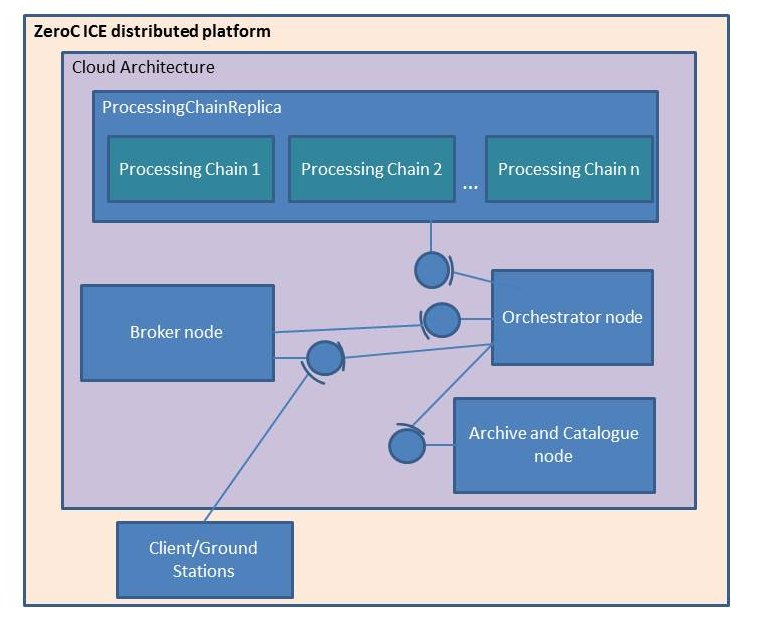
\includegraphics[width=0.95\textwidth]{cloud/second-architecture.jpg}
\caption{Cloud architecture using ZeroC ICE.}
\label{fig:ice-architecture}
\end{center}
\end{figure}


This architecture is independent of the platform when it is executed. There are
logical nodes in which ICE deploys the servers. These nodes may match with
physical nodes or may be several logical nodes in the same physical node. The
ICE runtime manages the location of the servers and their execution.

Furthermore, the data store is shared between all the servers. This means that the
components such as the \emph{Orchestrator}, the \emph{Archive and Catalogue} and the
\emph{Processing Chains} share the same logical memory space and they can write or read data
at the same time. This implementation avoids the file transfers and it does the
cloud infrastructure clearer, more dynamic and scalable.

In the following sections the  ICE interfaces between these components are
shown and the previous modules modules are explained. Their design and
interfaces with other modules are described. Finally, the
deployment of the software in each module is explained in detail.

\subsubsection{ICE interfaces}

The distributed application using ZeroC ICE was made using a slice file namely
``Geocloud.ice''for
specifying the  interfaces between components. These interfaces allows the transparently
communication between the components. The slice file is listed in Listing~\ref{code:ice-slice}.


\begin{listing}[
  float=h!,
  caption  = {Slice of the ICE application.},
  label    = code:ice-slice,
style=customc]

module geocloud {
    exception AlreadyExists { string key; };
    exception NoSuchKey { string key; };
    exception CreationScenarioException{};
    exception StartScenarioException{};
    exception StopScenarioException{};
    exception DeleteScenarioException{};
    exception ArchiveNotAvailableException{};
    exception OrchestratorNotAvailableException{};
    exception ProcessingException{};
    exception CataloguingException{};

    interface Orchestrator{
    	void initScenario(int scen) throws StartScenarioException,ArchiveNotAvailableException;
	void downloadedImage(string path);//the ground station calls this operation passing the path
	void imageProcessed(string path);
	void imageCatalogued(string path);
	void stopScenario() throws StopScenarioException;
    };

    interface Broker{
	void startScenario(int scen) throws OrchestratorNotAvailableException, StartScenarioException;
	void appendLog(string newLog);
	void stopScenario(int scen);
	void setOrchestrator( Orchestrator * orch);
	string getLastLogs();
    };


 interface Processor{
	//int init( Broker * log);
       	void processImage(string path) throws ProcessingException;
	void shutdown();
	void setOrchestrator(Orchestrator * orch);
    };



    interface ArchiveAndCatalogue{
	void createScenario(string scenario) throws CreationScenarioException;
	void catalogue(string path,string storage,string scenario) throws CataloguingException;
	void deleteScenario(int scenario) throws DeleteScenarioException;
    };
};
\end{listing}

\subsubsection{Implementation of the Orchestrator}

The \emph{Orchestrator} performs the same task that in the architecture based in
\ac{SSH} and \ac{SCP} (see Section~\ref{subsec:ssh-cloud}). It connects with the ground stations over \ac{FTP} connections and
then, the communications between the components of the cloud are done by using the
ICE interfaces of each component. ICE uses \ac{TCP} protocol by default.

\paragraph{Orchestrator Workflow}~\\

The \emph{Orchestrator} component works by following the next sequence of steps:
\begin{enumerate}
\item The ICE core application is initialized and the ICE communicator is
  created.
\item The \emph{Orchestrator Object Adapter} is instantiated and the \emph{Orchestrator} servant is
  added to it.
\item In the \emph{Orchestrator} initialization, the \emph{Listener} process is spawned.
\item The \emph{Listener} process creates the \emph{LoadData} object for loading the ground
  stations \ac{IP} addresses and the \ac{FTP} credentials.
\item The \emph{LoadData object} gets all the information about the \emph{Ground
    Stations Simulators} and localizes them.
\item The \emph{Listener} pools the \emph{Ground Stations} and when there are
  a downloadable raw data, the Orchestrator's function \emph{donwloadedImage} is
  called passing the absolute path of the image as parameter. 
\item  When the \emph{downloadedImage} is called, the \emph{Orchestrator}
  obtains the data.
\item  The \emph{Orchestrator} moves the raw data to a shared storage.
\item Then, the \emph{Orchestrator} makes different \emph{Job Orders} for the Processing Chains. The \emph{Job Order} contains all the required information by the \emph{Product Processing Chains} to proceed with the image processing.
\item The \emph{Orchestrator} gets the \emph{ProcessorChainReplica} proxy (this
  replica group contains all the Processing Chains in the cloud) and calls the
  \emph{processImage} operation of the proxy.
\item When the selected \emph{Processing Chain} finishes, it calls the \emph{processedImage}
  operation of the \emph{Orchestrator}.
\item The \emph{Orchestrator} obtains the \emph{Archive and Catalogue} proxy and
  sends the absolute path of the image for archiving and cataloguing.
\end{enumerate}

\paragraph{Orchestrator Interfaces}~\\

The \emph{Orchestrator} has interfaces with the Ground Stations implemented in
\emph{Virtual Wall}. Moreover this component  communicates with the \emph{Product Processing Chains} through the Replica
Group and with the
\emph{Archive and Catalogue}. 

\subparagraph{Interfaces with the Ground Stations implemented in Virtuall
  Wall}~\\

The \emph{Ground Stations} are deployed in some \emph{Virtual Wall} nodes. In
those, the impairments and features of the network are simulated. Essentially,
the \emph{Orchestrator} is pooling those \emph{Ground Stations} over \ac{FTP}
connections to know when new raw data is available. So, this Ground Stations are
\ac{FTP} servers in which the \emph{Orchestrator} can get the raw data recorded
by the constellation of satellites. 
As the ICE implementation could not be
deployed in the \bonfire platform, the checking and testing of funcionalities
were locally done. Thus, a client playing as a Ground Station was developed in
order to check and validate the architecture. 

\subparagraph{Interfaces with the  Processing Chains}~\\

The interfaces which the \emph{Processing Chains} provides are listed in
Listing~\ref{code:ice-slice}. The operations that the \emph{Orchestrator} uses
are \emph{processImage} and \emph{setOrchestrator} operations. 

\subparagraph{Interfaces with the Archive and Catalogue}~\\

The interfaces which the \emph{Archive and Catalogue} provides are listed in
Listing~\ref{code:ice-slice}. The operation that the \emph{Orchestrator} uses is
the \emph{catalogue} operation.


\paragraph{Orchestrator Design}~\\

The \emph{Orchestrator} module implements the \emph{Orchestrator} interface
which contains the following operations:
\begin{itemize}
\item \emph{void initScenario(int scen)}: it initializes the scenario in the
  module.
\item \emph{void downloadedImage(string path)}: it indicates to the
  \emph{Orchestrator} that an image is available to be processed  in the specified
  path.
\item \emph{void imageProcessed(string path)}: the Processing Chains call this function
  to indicate to the \emph{Orchestrator} that the processing of the image has
  finished, so the \emph{Orchestrator} can archive and catalogue it.
\item \emph{void imageCatalogued(string path)}: the catalogue module uses this
  function to notify the \emph{Orchestrator} that the image located in ``path'' was
  archived and catalogued.
\item \emph{void stopScenario(int scen)}: it stops the scenario in the
  \emph{Orchestrator}. Furthermore, it stops all the existing processing chains working.
\end{itemize}

The requests are served when they come to the \emph{Orchestrator} module. If
other request comes and the processing chains are busy, they are automatically queued by the
ICE execution core. Thus, it is not necessary to maintain a queuing algorithm in
the \emph{Orchestrator}. However it is necessary to have some data structures, in
this case dictionaries to temporaly store the images which are in different stages.

Furthermore, when the \emph{Orchestrator} is initialized the \emph{Listener} process is
accomplished. It listens the \ac{FTP} connections with the ground stations to detect and download new raw data. This process is always pooling the
ground stations until the \emph{Orchestrator} execution ends.

\paragraph{Orchestrator Implementation}~\\

The implementation of this module was done in Python 2.7 using ZeroC ICE 3.4. The
python's libraries needed to implement the software are listed in
Table~\ref{table:orches-second-libraries}

\begin{table}[hp]
  \centering
  {\small
  


\begin{tabular}{p{.2\textwidth}p{.2\textwidth}}
  \tabheadformat
  \tabhead{Python Library}   &
  \tabhead{Function}\\
\hline
\textit{Threading}         & System library for creating ,syncronizing and managing threads \\
\hline
\textit{OS}         & Library which provides operative system interactions \\
\hline
\textit{Collections}         & Library that contains the data structure
``deque'' used for queueing the request which can not be processed.\\
\hline
\textit{Time}         & For managing the time \\
\hline
\textit{Socket}         & Library for creating and establishing connections with other host \\
\hline
\textit{Pdb}         &  Used for debugging the software\\
\hline
\textit{FtpLib}         &Library used to obtain and manage the Ground Stations' FTP connections  \\
\hline
\end{tabular}


% Local variables:
%   coding: utf-8
%   ispell-local-dictionary: "castellano8"
%   TeX-master: "main.tex"
% End:

  }
  \caption{ICE \emph{Orchestrator} Python Libraries.}
  \label{table:orches-second-libraries}
\end{table}

\paragraph{OrchestratorExecution}~\\

To execute the \emph{Orchestrator} module the following dependencies
are required:
\begin{itemize}
\item \emph{ZeroC ICE 3.4} installed.
\item \emph Ethernet interface for connecting with the \emph{IceGrid} locator (see Section~\ref{subsub:deployment}).
\item \emph Configuration file for the node.
\end{itemize}
 In Section~\ref{subsub:deployment} the
  automatic deployment and execution of this module is explained. 

\subsubsection{Implementation of the  Processing Chain}

The \emph{Processing Chain} component processes the raw data to obtain a calibrated,
geolocated and orthorectified image. It executes all the product processor stages and notifies the
\emph{Orchestrator} server The background filesystem, where the cloud based in
ICE are implemented and executed, is a shared storage, so all the necessary files are
located in that shared memory space  explained in Section~\ref{par:pp-impl}. Moreover, all the instantiated \emph{Processing Chains} form part of the
\emph{ProcessingChainReplica} in order to provide load balancing and dynamic
replication services. 


\paragraph{Processing Chain Workflow}~\\

The \emph{Processing Chain} component works by following the next sequence of steps:

\begin{enumerate}
\item The \emph{setOrchestrator} operation is invoked for setting up the
  \emph{Orchestrator} in the \emph{Processing Chain}.
\item When the \emph{Orchestrator} invokes the \emph{processImage} fuction, the
  \emph{Processing Chain} starts to transform the raw data located in path.
\item When all the stages have been performed, the \emph{Processing Chain} calls the
  \emph{processedImage} of the \emph{Orchestrator}.
\item The \emph{Processing Chain} is ready for processing other image.
\item If the \emph{shutdown} function is called by the \emph{Orchestrator}, the
 \emph{Processing Chain} is turned off.
\end{enumerate}


\paragraph{Processing Chain Interfaces}~\\

The \emph{Processing Chain} component has interfaces with the \emph{Orchestrator}.

\subparagraph{Interfaces with the Orchestrator}~\\

The \emph{Processing Chain} server receives the order to process an image. When the
processing is finished, the \emph{Processing Chain} notifies the end of the
processing to the \emph{Orchestrator} by
calling the \emph{imageProcessed} function.

\paragraph{Processing Chain Design}~\\

The \emph{Processing Chain} module implements the \emph{Processor} interface, which
contains the following operations:

\begin{itemize}
\item \emph{void processImage(string path)}: it is invoked by the
  \emph{Orchestrator} in order to process the image located in path. Thus, all
  the product Processing Chains are sequentially executed and the \emph{processedImage}
  of the \emph{Orchestrator} is called. 
\item \emph{void shutdown()}: this funcion turns off the proccesor.
\item \emph{setOrchestrator()}: it sets up the \emph{Orchestrator} proxy to be
  used for the \emph{Processing Chain}.
\end{itemize}

\subparagraph{ProcessingChainReplica}~\\

This component involves all the \emph{Processing Chains} in the ICE application. It
provides two services: dynamic replication and load balancing. The first
of service is used for creating new on demand \emph{Processing Chains}. The second
one service servers the incoming petitions searching the less overloaded \emph{Processing Chain}
and returning its proxy for carrying out the request.

\paragraph{Processing Chain Implementation}~\\

The implementation of this module was done in Python 2.7 using ZeroC ICE 3.4. The
python's libraries needed to implement the software are listed in
Table~\ref{table:processor-second-libraries}.

\begin{table}[hp]
  \centering
  {\small
  


\begin{tabular}{p{.2\textwidth}p{.2\textwidth}}
  \tabheadformat
  \tabhead{Python Library}   &
  \tabhead{Function}\\
\hline
\textit{Threading}         & System library to create, syncronize and manage threads \\
\hline
\textit{OS}         & Library which provides operative system interactions \\
\hline
\textit{Pdb}         &  Used for debugging the software\\
\hline
\textit{Ice}         & ICE general purpose library \\
\hline
\textit{IceGrid}         & ICE library to use the IceGrid service \\
\hline
\end{tabular}


% Local variables:
%   coding: utf-8
%   ispell-local-dictionary: "castellano8"
%   TeX-master: "main.tex"
% End:

  }
  \caption{ICE Processor Python Libraries.}
  \label{table:processor-second-libraries}
\end{table}

\paragraph{Processing Chain Execution}~\\

To execute the \emph{Processing Chain} module the following dependencies
are required:
\begin{itemize}
\item \emph{ZeroC ICE 3.4} installed.
\item \emph Ethernet interface for connecting with \emph{IceGrid} locator.
\item \emph Configuration file for the node. In Section~\ref{subsub:deployment} the
  automatic deployment of the \emph{Processing Chain} and its execution are explained. 
\end{itemize}

\subsubsection{Implementation of the Archive and Catalogue}

The implementation of the \emph{Archive and Catalogue} component using
ZeroC ICE was
performed to archive and catalogue the processed images. It uses the
\emph{GeoServer} software and the Python library (Gsconfig) to catalogue and
archive the images.

\paragraph{Archive and Catalogue Workflow}~\\

The \emph{Archive and Catalogue} component works by following the next sequence of steps:
\begin{enumerate}
\item The ICE core application is initialized and the ICE communicator is
  created.
\item The \emph{Archive and Catalogue Object Adapter} is instantiated and the \emph{A\&C} servant is
  added to it.
\item When the initialization of a scenario is called, a workspace is created.
\item Then, when a image is requested for cataloguing, the module communicates with the
  \emph{GeoServer} software by the library to catalogue. 
\item The images are catalogued in the same workspace.
\item When the scenario ends, \emph{deleteScenario} is invoked and the
  workspace is deleted.
\end{enumerate}

\paragraph{Archive and Catalogue Interfaces}~\\

The \emph{Archive and Catalogue} module has interfaces with the
\emph{Orchestrator} and the \emph{GeoServer} software.

\subparagraph{Interfaces with the Orchestrator}~\\

The \emph{Archive and Catalogue} module notifies a images was catalogue to the \emph{Orchestrator} by
using the \emph{imageCatalogued} call when a
image is catalogued.

\subparagraph{Interfaces with the GeoServer software}~\\

The \emph{GeoServer} software provides a Python library named
\emph{Gsconfig}. The official page of this library is
\url{https://github.com/boundlessgeo/gsconfig}. Using this library, operations
with layers, images, tilesets or storages can be done. The provided operations
for cataloguing ``tiff'' images (the default format for geodata images) were
used.

\paragraph{Archive and Catalogue Design}~\\

The \emph{Archive and Catalogue} module implements the \emph{Archive and
  Catalogue} interface, which contains the following operations:

\begin{itemize}
\item \emph{void createScenario(string scenario)}: it is invoked by the
  \emph{Orchestrator} and creates the workspace into the \emph{GeoServer}
  platform for storing the images.
\item \emph{void catalogue(string path, string storage,string scenario)}: It
  catalogues the image located in path, it creates the storage where the image is
  stored and it creates the workspace named scenario.
\item \emph{void deleteScenario(string scenario)}: it deletes the workspace created
  to carry out the experiment.
\end{itemize}


\paragraph{Archive and Catalogue Implementation}~\\

The implementation of this module was done in Python 2.7 using ZeroC ICE 3.4. The
python's libraries needed to implement the software are listed in
Table~\ref{table:ayc-second-libraries}.

\begin{table}[hp]
  \centering
  {\small
  


\begin{tabular}{p{.2\textwidth}p{.2\textwidth}}
  \tabheadformat
  \tabhead{Python Library}   &
  \tabhead{Function}\\
\hline
\textit{Time}         & To manage the time \\
\hline
\textit{Pdb}         &  Used for debugging the software\\
\hline
\textit{Gsconfig}         &Library used to communicates with \emph{GeoServer} software \\
\hline
\textit{Ice}         & ICE general purpose library \\
\hline
\textit{IceGrid}         & ICE library to use the IceGrid service \\
\hline
\end{tabular}


% Local variables:
%   coding: utf-8
%   ispell-local-dictionary: "castellano8"
%   TeX-master: "main.tex"
% End:

  }
  \caption{ICE \emph{Archive and Catalogue} Python Libraries.}
  \label{table:ayc-second-libraries}
\end{table}

The \emph{Gsconfig} library was manually installed as follows:
\begin{itemize}
\item The library is obtained from the following url: \url{https://github.com/boundlessgeo/gsconfig}.
\item Firstly, the ``Python-pip''  package is installed.
\item Then just execute ``pip install gsconfig''.
\end{itemize}

The \emph{GeoServer} software was required to be installed. For that purpose, the
\emph{Apache Tomcat} server was installed. Then, the ``war''
file which contains the \emph{GeoServer} software was downloaded from the
official webpage and it was installed into the \emph{Tomcat} server.

\paragraph{Archive and Catalogue Execution}~\\

To execute the \emph{Orchestrator} module, the following dependencies
are required:
\begin{itemize}
\item \emph{ZeroC ICE 3.4} installed.
\item \emph Ethernet interface for connecting with the \emph{IceGrid} locator (see
  Section~\ref{subsub:deployment}).
\item \emph{Apache Tomcat}.
\item \emph{Geoserver with the \ac{CSW} plugin}.
\item \emph{Gsconfig library installed}.
\item \emph Configuration file for the node.
\end{itemize}
 In Section~\ref{subsub:deployment} the
  automatic deployment and execution of the \emph{Archive and Catalogue} is explained. 

\subsubsection{Implementation of the Broker}

The \emph{Broker} component performs the initialization and the stop of the
experiments. In addition, it collects the which are accesible by the experimenters.

\paragraph{Broker Workflow}~\\

The \emph{Broker} component works by following  sequence of steps:
\begin{enumerate}
\item The ICE core application is initialized and the ICE communicator is
  created.
\item The \emph{Broker Object Adapter} is instantiated and the \emph{Broker} servant is
  added to it.
\item The  \emph{Broker} creates a data structure for storing the last log
  received.
\item The \emph{Broker} receives a log and it stores it in the data structure.
\item When the \emph{Broker} receives a request applying for the logs, the
  \emph{Broker} returns them and it cleans the data structure.
\item When the experimenter invokes the \emph{startScenario} of the \emph{Broker}, it
  obtains the \emph{Orchestrator} proxy and it calls the remote method
  \emph{initScenario} of the \emph{Orchestrator} interface.
\item When the experimenter invokes the \emph{stopScenario} of the \emph{Broker}, it
  obtains the \emph{Orchestrator} proxy and it calls the remote method
  \emph{stopScenario} of the \emph{Orchestrator} interface.
\end{enumerate}

\paragraph{Broker Interfaces}~\\

The \emph{Broker} component has interfaces with the \emph{Orchestrator}, with
all the cloud components and with the clients used by experimenters.

\subparagraph{Interfaces with the Orchestrator}~\\

The \emph{Broker} module communicates with the \emph{Orchestrator} by using the
\emph{initScenario} and \emph{stopScenario} calls. The first one is used to
initialize the experiment in the \emph{Orchestrator} and the second one is used
to stop the experiment in the \emph{Orchestrator}.

\subparagraph{Interfaces with all the cloud components}~\\

The cloud components communicate with the \emph{Broker} by using the
\emph{appendLog} operation. When this operation is invoked, the log sent as parameter is added in the log data structure.  

\subparagraph{Interfaces with the clients}~\\

The clients invokes the \emph{getLastLogs} procedure in order to obtains
all the logs collected.

\paragraph{Broker Design}~\\

The \emph{Broker} module implements the \emph{Broker} interface which
contains the following operations:

\begin{itemize}
\item \emph{void startScenario(int scen)}: it initializes the data structure to
  store logs and initializes the \emph{Orchestrator} by calling \emph{initScenario}.
\item \emph{void stopScenario(int scen)}: it calls the \emph{stopScenario}
  operation of the \emph{Orchestrator}. The data structure is not cleaned in
  this method because all the available logs may not be read by the experimenter
  client.
\item \emph{void appendLog(string log)}: this function is called by all
  components of the  cloud and it appends the log as parameter in the data
  structure of the \emph{Broker}. 
\item \emph{string getLastLogs()}: this function returns to the applicant client
  the last available logs in the log data structure. When finished, the log structure is
  cleaned for appending more log strings.
\item \emph{void setOrchestrator( Orchestrator *orch )}: it sets up the
  \emph{Orchestrator} proxy passed as parameter to be
  used by the \emph{Broker}.
\end{itemize}


\paragraph{Broker Implementation}~\\

The implementation of the \emph{Broker} was done in Python 2.7 using ZeroC ICE 3.4. The
python's libraries needed to implement the software are listed in
Table~\ref{table:broker-libraries}

\begin{table}[hp]
  \centering
  {\small
  


\begin{tabular}{p{.2\textwidth}p{.2\textwidth}}
  \tabheadformat
  \tabhead{Python Library}   &
  \tabhead{Function}\\
\hline
\textit{Time}         & For managing the time \\
\hline
\textit{Pdb}         &  Used for debugging the software\\
\hline
\textit{Ice}         & ICE general purpose library \\
\hline
\textit{IceGrid}         & ICE library to use the IceGrid service \\
\hline
\end{tabular}


% Local variables:
%   coding: utf-8
%   ispell-local-dictionary: "castellano8"
%   TeX-master: "main.tex"
% End:

  }
  \caption{ICE Broker Python Libraries.}
  \label{table:broker-libraries}
\end{table}


\paragraph{Broker Execution}~\\

To execute the \emph{Broker} module the following dependencies
are required:
\begin{itemize}
\item \emph{ZeroC ICE 3.4} installed.
\item \emph Ethernet interface for connecting with \emph{IceGrid} locator.
\item \emph Configuration file for the node. In Section~\ref{subsub:deployment} the
  automatic deployment and its execution of the \emph{Broker} are explained. 
\end{itemize}


\subsubsection{Implementation of the client}

The client developed for testing and checking the funcionality of the cloud
architecture were developed in the ICE runtime environment. The functionalities
that the client performs are the following:
\begin{itemize}
\item Obtaining the \emph{Orchestrator proxy}.
\item Sending raw data to  \emph{Orchestrator} by calling \emph{downloadedImage}.
\item Calling \emph{getLastLogs} function of the \emph{Broker}, periodically.
\end{itemize}

As future work, the ground stations may be implemented by using the ICE
middleware. It would provide more transparency and easiness to deploy the
experiments. Furthermore, it would facilitate the integration with the
\emph{Orchestrator} by using the \emph{Orchestrator} interface to notify that
there are new raw data availble.

The implementation of this module was done in Python 2.7 using ZeroC ICE 3.4. The
python's libraries needed to implement the software are listed in
Table~\ref{table:client-libraries}

\begin{table}[hp]
  \centering
  {\small
  


\begin{tabular}{p{.2\textwidth}p{.2\textwidth}}
  \tabheadformat
  \tabhead{Python Library}   &
  \tabhead{Function}\\
\hline
\textit{Pdb}         &  Used for debugging the software\\
\hline
\textit{Ice}         & ICE general purpose library \\
\hline
\textit{IceGrid}         & ICE library to use the IceGrid service \\
\hline
\end{tabular}


% Local variables:
%   coding: utf-8
%   ispell-local-dictionary: "castellano8"
%   TeX-master: "main.tex"
% End:

  }
  \caption{ICE Client Python Libraries.}
  \label{table:client-libraries}
\end{table}

\paragraph{Client Execution}~\\

To execute the client attached in the CD-ROM, the following dependencies
are required:
\begin{itemize}
\item \emph{ZeroC ICE 3.4} installed.
\item \emph Ethernet interface for connecting with \emph{IceGrid} locator (see
  Section~\ref{subsub:deployment}.
\item \emph Configuration file for the locator.
\end{itemize}

The execution of the client, which is located in ``source/ice/src/client.py'',
is done as follows:
\begin{itemize}
\item[>] python client.py --Ice.Config=cfg/locator.cfg
\end{itemize}


\subsubsection{Deployment of the ICE architecture}
\label{subsub:deployment}

The deployment of the ICE architecture was done using the \emph{IceGrid}
and \emph{IcePatch} services. 
\emph{IceGrid} provides location transparency by using well-known objects and server replication and load
balancing services by creating replica groups. \emph{IcePatch} is an
efficient file patching service which is easy to configure and use. It provides the
automatically source distribution to all nodes.

The deployment was made creating a distributed application (located in
``source/ice/app'' folder) which is composed by
nodes, servers running in the nodes and object adapters created by the servers. 
The nodes are the logical implementation of a physical node where any kind of
server can be executed. The nodes created for this deployment were the
following:

\begin{itemize}
\item \emph{Orchestrator node}: it contains the \emph{Orchestrator} server.
\item \emph{Archive and Catalogue node}: it contains the \emph{Archive and Catalogue}
  server. The \emph{GeoServer} software is also included.
\item \emph{Broker node}: it contains the \emph{Broker} server which acts as an
  intermediate between the cloud architecture and the client or ground stations.
\item \emph{Processing Chain node}: it contains a \emph{Processing Chain} server. 
\end{itemize}


Some scripts for initializing the nodes were developed. This scripts are the
following: 
\begin{itemize}
\item Start.sh: it creates the folder structure and launches the
  ``icegridnode'' daemons for each node.
\item Stop.sh: it stop the nodes.
\item Clean.sh: it cleans the temporaly files and directories created during the execution.
\end{itemize}

Moreover, the source must be located in ``/tmp/ice'' because to create an application for
deploying in several machines, the most usual is to provide a way for an easy
deployment. 

For the deployment was effective, the ``icegridnode'' services must be running
in each node. 
There are several configuration files for the nodes. These files are located in\\
``source/ice/cfg/'' directory. The ``node\$.cfg'' files ,where ``\$'' is a number,
are the configuration files for the nodes. One of them, in this case the
``node1.cfg'' contains the configuration for the locator service. 
The locator service provides to ICE applications the location of all well-known
objects registered in the ICE runtime environment. 
The execution of each node is done as follows:
\begin{itemize}
\item[>]icegridnode --nochdir --daemon --Ice.Config=cfg/nodo\$.cfg
\end{itemize}
where \$ is the number of node to be executed.
 
Finally the installation of the application and the source distribution is done
by the following command:
\begin{itemize}
\item[>]icegridadmin --Ice.Config=cfg/locator.cfg -e ``application add
  app/GeoCloudApp.xml''
\end{itemize}

where the locator file contains the address of the node where it is located and
the \emph{GeoCloudApp.xml} is the application description where the deployment,
replication policies and the different services involve in the distributed
application are defined. Executing the \emph{icegridadmin} command and
installing the application, automatically are deployed and started up the
servers in their respective node.

